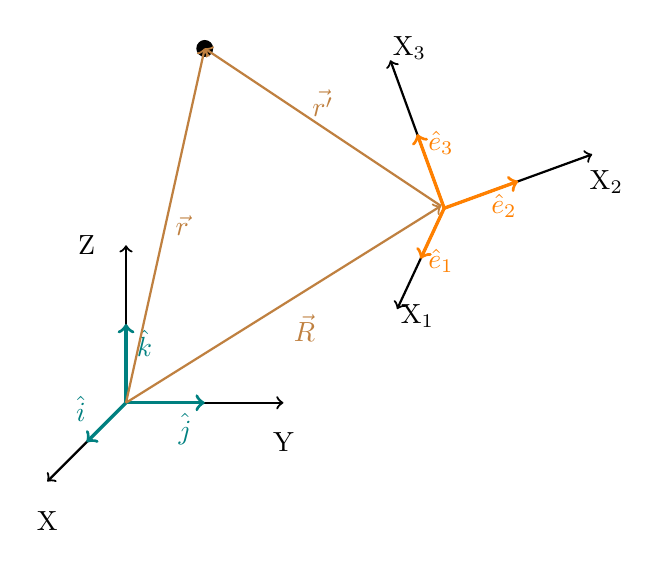
\begin{tikzpicture}
\draw [fill] (1,3.5) circle (0.1);
\draw [<->, thick] (0,1) -- (0,-1) node (v1) {} -- (2,-1);
\draw [->, thick] (v1.center) -- (-1,-2);
\node at (-1,-2.5) {X};
\node at (2,-1.5) {Y};
\node at (-0.5,1) {Z};
\draw [->, very thick, teal] (v1.center) -- (-0.5,-1.5) node [near end, above left]{$\hat{i}$};
\draw [->, very thick, teal] (0,-1) node (v2) {} -- (0,0)node [near end, right]{$\hat{k}$};
\draw [->, very thick, teal] (v2.center) -- (1,-1)node [near end, below]{$\hat{j}$};
\draw [->, thick, brown](v2.center) -- (4,1.5) node [midway, below right]{$\vec{R}$};
\draw [->, thick, brown](v2.center) -- (1,3.5)node [midway, right]{$\vec{r}$};
\draw [->, thick, brown](4,1.5) -- (1,3.5)node [midway, above]{$\vec{r'}$};
\draw [<->, thick, rotate =20] (4.3,2) -- (4.3,0)  -- (6.3,0);
\draw [->, thick, rotate =20] (4.3,0) node (v3) {} -- (3.3,-1);
\node at (3.7,0.1) {X$_1$};
\node at (6.1,1.8) {X$_2$};
\node at (3.6,3.5) {X$_3$};
\draw [<->, very thick, orange, rotate =20](4.3,1) -- (v3.center) -- (5.3,0);
\draw [->, very thick, orange, rotate =20](v3.center) -- (3.8,-0.5);
\node at (4,0.8) [orange]{$\hat{e}_1$};
\node at (4.8,1.5) [orange]{$\hat{e}_2$};
\node at (4,2.3) [orange]{$\hat{e}_3$};

\end{tikzpicture}